\documentclass{article}
\usepackage{arxiv}

\usepackage[utf8]{inputenc}
\usepackage[english, russian]{babel}
\usepackage[T1]{fontenc}
\usepackage{url}
\usepackage{booktabs}
\usepackage{amsfonts}
\usepackage{nicefrac}
\usepackage{microtype}
\usepackage{lipsum}
\usepackage{graphicx}
\usepackage{natbib}
\usepackage{doi}
\usepackage[table]{xcolor}

% \usepackage[
% backend=biber,
% style=alphabetic,
% sorting=ynt
% ]{biblatex}


\title{GraphSASRec: модель последовательных рекомендаций на основе самовнивания, дополненная графовыми представлениями.}

\author{ 
	\textbf{Матвеев Артем} \\
    Московский государственный университет \\ 
	имени М. В. Ломоносова \\
	\texttt{matfu21@ya.ru} \\
	\And
	\textbf{Майсурадзе Арчил Ивериевич} \\
    Московский государственный университет \\
	имени М. В. Ломоносова \\
	\texttt{artchil@mail.ru} \\
}
\date{2023}

\renewcommand{\shorttitle}{}

\begin{document}
\maketitle

\begin{abstract}
	% \lipsum[1]
	Последовательные модели, решающие задачу предсказания следующего взаимодействия пользователя на 
	основе кодирования его исторических событий, являются популярным решением для построение 
	персонализированных рекомендательных систем как в индустрии, так и в академии. Преимуществами 
	таких моделей являются: учет порядка, в котором следуют исторические события и оценка долгосрочных 
	интересов пользователя. Однако подобные подходы недостаточно эксплуатируют полезный коллаборативный
	сигнал и плохо представляют объекты из длинного хвоста. Популярным решением этих проблем являются 
	методы, основанные на применении графовых нейронных сетей к двудольному графу взаимодействий 
	пользователей. В работе предлагается с другой стороны взглянуть на модель последовательных рекомендаций
	как на графовую сеть со стороны пользователя. Предлагается метод увеличения глубины этой сети,
	сохраняющий длину истории пользователя при минимальных накладных расходах. Предлагается способ корректировки
	смещения, вызванного семплированием из показательного распределения для задачи link-prediction. 
	Наблюдаемые результаты демонстрируют улучшение с точки зрения метрик ранжирования и разнообразия выдачи.
\end{abstract}


\keywords{Информационный поиск \and Последовательные рекомендации \and Графовые нейронные сети}

\section{Введение}

Последовательные рекомендательные системы - это класс рекомендательных систем, которые принимают 
во внимание порядок взаимодействий пользователя и пытаются предсказать следующее его взаимодейсвие.
Учет порядка является важной состоявляющей во многих рекомендательных сценариях: если пользователь
только что купил мобильный телефон, то следующая покупка с большой долей вероятности будет 
аксессуаром к нему. Ранее такая задача решалась с помощью подходов, основанных на Марковских 
цепях \cite{mc} или рекуррентных нейронных сетях \cite{rnn1,rnn2,rnn3}. Но после появления архитектуры
трансформер \cite{transformer} и его успеха в задачах распознования естественного языка, наиболее успешными
стали модели, основанные на обработке последовательностей действий пользователя с помощью трансформера 
\cite{sasrec,bert4rec,gsasrec}. 

Другим популярным подходом в рекомендательных системах являются графовые нейронные 
сети \cite{lightgcn,lightgcl,hetergcl,herograph,slgcn}. В этом подходе информация, которая есть в рекомендательной 
системе, рассматривается в виде графов. Большинство данных в любой рекомендательной системе по
существу имееют графовую структуру. Например, данные взаимодействий в рекомендательном сервисе могут быть
представлены в виде двудольного графа, вершины одной доли которого - пользователи, другой объекты (например, товары), а
наблюдаемый взаимодействия - ребра. Пусть нам дан такой граф. Ключевая идея графовых нейронный сетей заключается в
итеративной агрегации признаковых представлений соседей в графе и объединение этой агрегированной информации
с представлением вершины, для которой рассматривается соседство \cite{survey1}. Такая операция называется распространением
сообщений \cite{lightgcn,sage}. Формально ее можно записать в следующем виде:$$
Aggregation: n^{(l)}_v = Aggregator_l(\{h^l_u, \forall u \in \mathcal{N}_v\}),$$$$Update: h^{(l + 1)}_v = Updater_l(h_v^{(l)}, n_v^{(l)}),
$$ где $h_u^{(l)}$ определяется как представление вершины $u$ после $l$-ого слоя графовой сети. $Aggregator_l$ и $Update_l$
представляют собой обучаемые функции агрегации соседей и обновления представления вершины на $l$-ом слое. В качестве функции 
агрегации могут выступать как простые варианты по типу max-pooling, mean-pooling \cite{sage}, так и более сложные, например: 
importance-pooling \cite{pinsage}, агрегация на основе контекста \cite{multisage}, механизм внимания \cite{gat}, агрегация
на базе трансформера \cite{multibisage}. В качестве функции обновления могут выступать как простые архитектуры на базе несколькоих
полносвязных слоев \cite{sage, pinsage}, так и более сложные на базе трансформера \cite{multibisage}.

Успех графовых подходов в рекомендательных системах можно объяснить тремя причинами \cite{survey2}. Во-первых,
выражая все данные в виде вершин и ребер графа, графовые нейронные сети предоставляют общий способ
использовать все имеющиеся данные \cite{twhin}, тогда как традиционные рекомендательные системы чаще
всего фокусируются на одном или небольшом количестве источников данных. Во-вторых, подобные модели могут явно
утилизировать связи высокого порядка (товар $X$ купил пользователь $U$, которому понравился товар $Y$, который в свою очередь
похож на товар $Z$). В классических моделях этот учет происходит только неявно. Причем многие работы показывают, что от увеличения
глубины графовой сети (то есть явного учета взаимодействий более высокого порядка) наблюдается рост целевых 
метрик \cite{lightgcn,sage,podcastgnn}. В-третьих, целевой сигнал в рекомендательных системах очень 
разреженный (например, покупка). Графовые подходы позволяют использовать методы, основанные на обучении с частичным 
привлечением учителя \cite{semisupervised}, что приводит к улучшению качества моделей.

При внимательном взгляде на модели последовательных рекомендаций, можно увидеть в них графовую нейронную
сеть со стороны пользователя. Как было упомянуто выше, графовые нейронные сети выучивают лучшее 
семантическое пространство, если начинать использовать в модели связи все большего порядка. Однако, на практике,
длина последовательности пользователя варьируется от сотен \cite{sasrec,yandex}, до тысяч \cite{pinnerformer,transact}
исторических событий. В этом случае, при построении соседств следующих уровней, возникает проблема
экспоненциального роста их размера \cite{sage}, что приводит к невозможности применения графовых методов 
в классическом виде.

Основной вклад заключается в следующем:

\begin{enumerate}
	\item[\textbullet] Предлагается с другой стороны взглянуть на задачу последовательных рекомендаций. Найти в ней сходства с подходами, связанными с графовыми
нейронными сетями, и использовать методы из этой области для улучшения моделей последовательных рекомендаций.
	\item[\textbullet] Предлагается метод увеличения глубины связей, утилизируемых в моделях последовательных рекомендаций, на оснвое 
предобученных графовых представлений. При этом сохраняющей длину истории пользователя при минимальных накладных расходах.
	\item[\textbullet] Представляется способ корректироваки, получающий асимптотически несмещенную оценку градиента для функции потерть в задаче link-prediction. 
Приводятся результаты, демонстрирующие улучшения с точки зрения метрик полноты по сравнению с решением, не использующим эту корректировку.
	\item[\textbullet] Представляется модифицированная архитектура модели последовательных рекомендаций, учитывающая связи более высоких порядков. Демонстрируются
результаты, показывающие, что такой подходи приводит к росту метрик ранжирования. 
\end{enumerate}
 

\section{Постановка задачи}

\subsection{Последовательные рекомендации}
В последовательных рекомендациях рассматривается задача предсказания следующего положительного взаимодействия 
пользователя по последовательности его исторических действий $S^u = (S_1^u, S_2^u, \dots, S_{|S^u|}^u)$.
Во время обучения, на момент времени $t$, модель предсказывает следующий объект интереса пользователя на основе его
взаимодействий, произошедших раньше момента $t$. На вход модели поступает последоватлеьность
$(S_1^u, S_2^u, \dots, S^u_{|S^u| - 1})$. Ожидаемый выход модели - следующее положительное взаимодействия $S^u_{|S^u|}$. 
В данной работе рассматривается модель SASRec \citep{sasrec}, в основе которой лежит декодер блок трансформера \cite{transformer},
на выходе которого тоже последовательность. 
Поэтому задачу можно переформулировать в эквивалентном виде, как задачу предсказания сдвинутой версии 
последовательности $(S_2^u, S_3^u, \dots, S^u_{|S^u|})$.

\subsection{Предсказание ребра}

Дан граф $G = (V, E, X)$, где $V$ - множество вершин, $E$ - множество ребер, $X \in \mathbb{R}^{|V| \times d}$
- $d$-размерные векторные представления входных вершин. Задача предсказания ребра формулируется как задача
определения существования (или появления в будущем, если граф рассматривается как динамический \cite{dyngnn}) ребра $e_{ij}$
между вершинами $i$ и $j$, где $i, j \in V$, и $e_{ij} \not \in E$.

\section{Сопутствующие работы}

\subsection{Последовательные рекомендации в индустрии}

В реальных рекомендательных системах процесс получения кандидатов для пользователя разбивается на две части: матчинг и ранжирование.
На стадии матчинга применяются относительно легкие модели \cite{xwalk,logQ}, которые из миллионов-миллиардов кандидатов отбирают сотни-тысячи. 
На стадии ранжирования применяются тяжелые модели \cite{dcnv2,masknet,catboost}, уточняющие прогнозы моделей с предыдущей стадии. Модели
последовательных рекомендаций применяются на обоих стадиях. Например, модель PinnerFormer \cite{pinnerformer} применяется на стадии 
матчинга. Ее особенность заключается в том, что предсказывается не просто следующее взаимодействие пользователя, а сразу несколько следующих
взаимодействий, что позволяет учитывать долгосрочные интересы пользователя. Примером модели, которая применяется на стадии ранжирования является
UserBody \cite{yandex}. Ее особенность заключается в двух стадиях обучения: предобучение и дообучении. Предобучение происходит на стандарную для
матчинга Sampled-Softmax функцию потерь. Дообучения происходит на задачу ранжирования с классическим попарным лоссом в качестве оптимизируемого критерия.

\subsection{Графовые подходы в индустрии}

В большинстве академических работ в моделях на основе графов каждой вершине ставится в соответствие обучаемый вектор \cite{lightgcn}. 
Дальше такие модели учатся совместно с этими векторами. Минусом таких моделей является невозможность обобщения на новые вершины, 
которые со временем появляются в графе. Модели, обладающие таким свойством, называются трансдуктивными. Еще одним минусом транcдуктивного
подхода являются огромные матрицы эмбеддингов, совпадающие по размеру с количеством вершин в графе. Это приводит к резкому росту
числа параметров модели. Уже при миллионах вершин размеры моделей будут исчисляться миллиардами параметров, тогда как на практике количество
вершин в графах может достигать и десятков миллиардов. Такой рост числа параметров приводит к необходимости использовать разреженные
методы оптимизации (SparseAdam), что приводит к худшей траектории оптимизации. Именно поэтому в данной работе предлагается фокусироваться
на подходах из индустрии.

В противовес к трансдуктивным графовым подходам выделяются индуктивные \cite{sage}. Их особенность заключается в том, что во настройки модели
выучивается только преобразование над входными данными, что приводит к способности обобщаться на новые данные, которых раньше не было в обучающей выборке.

В индустрии можно выделить два подхода к добавлению графовой информации к моделям: end-to-end обучение вместе с целевой задачей и переиспользование
заранее предобученных графовых векторов в последующих моделях для матчинга и ранжирования. Второй подход в свою очередь разбивается на два: трансдуктивные
и индуктивные модели для получения предобученных графовых векторов.

\subsection{End-to-end подходы}

В подходе от Etsy \cite{etsy} рассматривается двухбашенная модель для задачи матчинга в товарном поиске. Выбирается двудольных граф запрос-товар, где ребро 
проводится в случае, если с поискового запроса был переход на товар. Графовая структура здесь учитывается следующим образом: в башню над товаром дополнительно подаются запросы, 
связанные с товаром в двудольном графе. Т.к. таких запросов может быть много, семплируется фиксированное количество, а дальше это соседство агрегируется с помощью
усреднения. Похожие подходы используются у Amazon \cite{amazon} и Taobao \cite{taobao}. Еще один подход от Alibaba Group \cite{alibaba} заключается в том, чтобы на стадии 
обучения сближать представления, выдаваемые моделью последовательных рекомендаций с графовыми представлениями с помощью 
контрастивного обучения, тем самым заставляя модель выучивать неявным образом графовую структуру.


\subsection{Транcдуктивные графовые модели}

Как уже было сказано выше, трансдуктивные модели обладают рядом недостатков, что делает их обслуживание в реальных системах затруднительным.
Однако одним из успешных примеров трандуктивной модели в индустрии является TwHIN \cite{twhin} от Twitter. В основе TwHIN лежит модель TransE \cite{transe},
в которой каждой вершине и каждому типу ребра присваивается свой обучаемый вектор. Для обучения такой модели используется специальный фреймворк PyTorch-BigGraph \cite{biggraph},
который использует специальный механизм бакетирования, позволяющий работать с огромными матрицами эмбеддингов. Обучения векторов происходи на задачу 
link-prediction. Полученные предобученные векторы далее используются во всех рекомендательных моделях Twitter в замороженном виде как источник графовой структуры \cite{twhinbert,twerc}.
Другим примером использования трандуктивной модели является Spotify \cite{spotify}.

\subsection{Индуктивные графовые модели}

Самым успешным примером индуктивного подхода является Pinterest: PinSage \cite{pinsage}, MulitSage \cite{multisage}, MultiBiSage \cite{multibisage}. Получившиеся 
предобученные векторы далее используются в задача матчинга \cite{pinnerformer}, ранжирования \cite{transact} и получении новых векторов \cite{itemsage}.
Похожие работы есть у Spotify \cite{podcastgnn}, Amazon \cite{amazonalexa} и Walmart \cite{walmart}.

\section{Метод}

Кратко, предлагаемый метод заключается в следующем:
\begin{enumerate}
	\item[\textbullet] Строится двудольных граф взаимодействий пользователей с объектами.
	\item[\textbullet] На основе этого графа выучиваются векторные представления вершин на задачу предсказания ребра (link-prediction).
	\item[\textbullet] Предобученные векторные представления с помощью преобразования с нелинейностью переводятся в одно семантическое пространство
с обучаемыми векторами для объектов из модели SASRec. К каждому объекту исторической последовательности прибавляется преобразованный графовый вектор.
Преобразование над предобученными графовыми векторами обучается вместе с моделью SASRec на задачу предсказания следующего положительного взаимодействия
пользователя (см. Рис. 1).
\end{enumerate}

\texttt{Предобученные графовые векторы.} В качестве модели, получающей предобученные графовые представления, будет выступать
GraphSAGE \cite{sage}. Формально, в общем случае, метод можно представить в следующем виде:

$$
h^k_{\mathcal{N}(v)} \leftarrow AGGREGATE_k(\{h^{k - 1}_u, \forall u \in \mathcal{N}(v)\}),
$$
$$
h^k_v \leftarrow \sigma(W^k \cdot CONCAT(h^{k - 1}_v, h^k_{\mathcal{N}(v)})), 
$$
$$
z_v \leftarrow \frac{h_v^k}{||h^k_v||_2}.
$$


Особенностью метода GraphSAGE является семплирование соседства для каждой вершины, что приводит к борьбе с экспоненциальным ростом размера окрестности.
Для получения эмбеддингов вершин будет рассматриваться только соседство первого уровня. 
Обучения происходит в постановке обучения без учителя на предсказание ребра в этом графе. Функция потерь в этому случае
выглядит следующим образом:

$$
\mathcal{L}(u, i) = - \log(\sigma(z_u^T z_v)) - \mathbb{E}_{v_n \sim P_n(v)} \log (\sigma(-z^T_u z_{v_n})).
$$

Матожидание оценивается по Монте-Карло. На практике, семплирование происходит по негативным примерам из очередного батчка, что приводит
к смещенной оценке. Решением этой проблемы является корректировка, представленная в секции 5.

\begin{figure}[!ht]
    \centering
    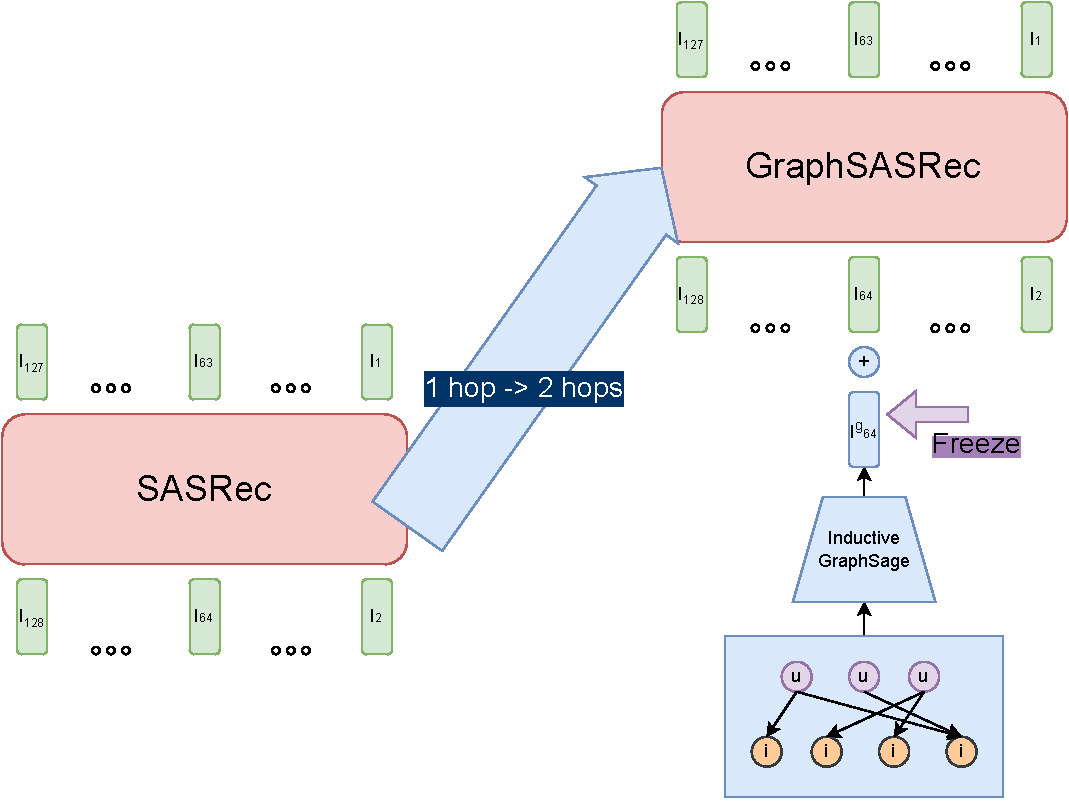
\includegraphics[width=150mm]{images/grpahsasrec2.pdf}
    \caption{Переход от модели SASRec к GraphSASRec.}
\end{figure}

\texttt{GraphSASRec.} Модель отличается от SASRec добавлением графовых векторов. Целевая задаче не меняется, все та же бинарная кросс-энтропия.

\section{Корректировка смещения, вызванного семплированием}

Как было сказано выше, если проводить оптимизацию на канонический link-prediction, в котором негативные примеры семплируются в рамках батча:
$$
Link-prediction = - \frac{1}{2 bs} (\sum_{j = 1}^{bs})
$$
, где $bs$ - размер очередного батча.
\begin{figure}[!ht]
    \centering
    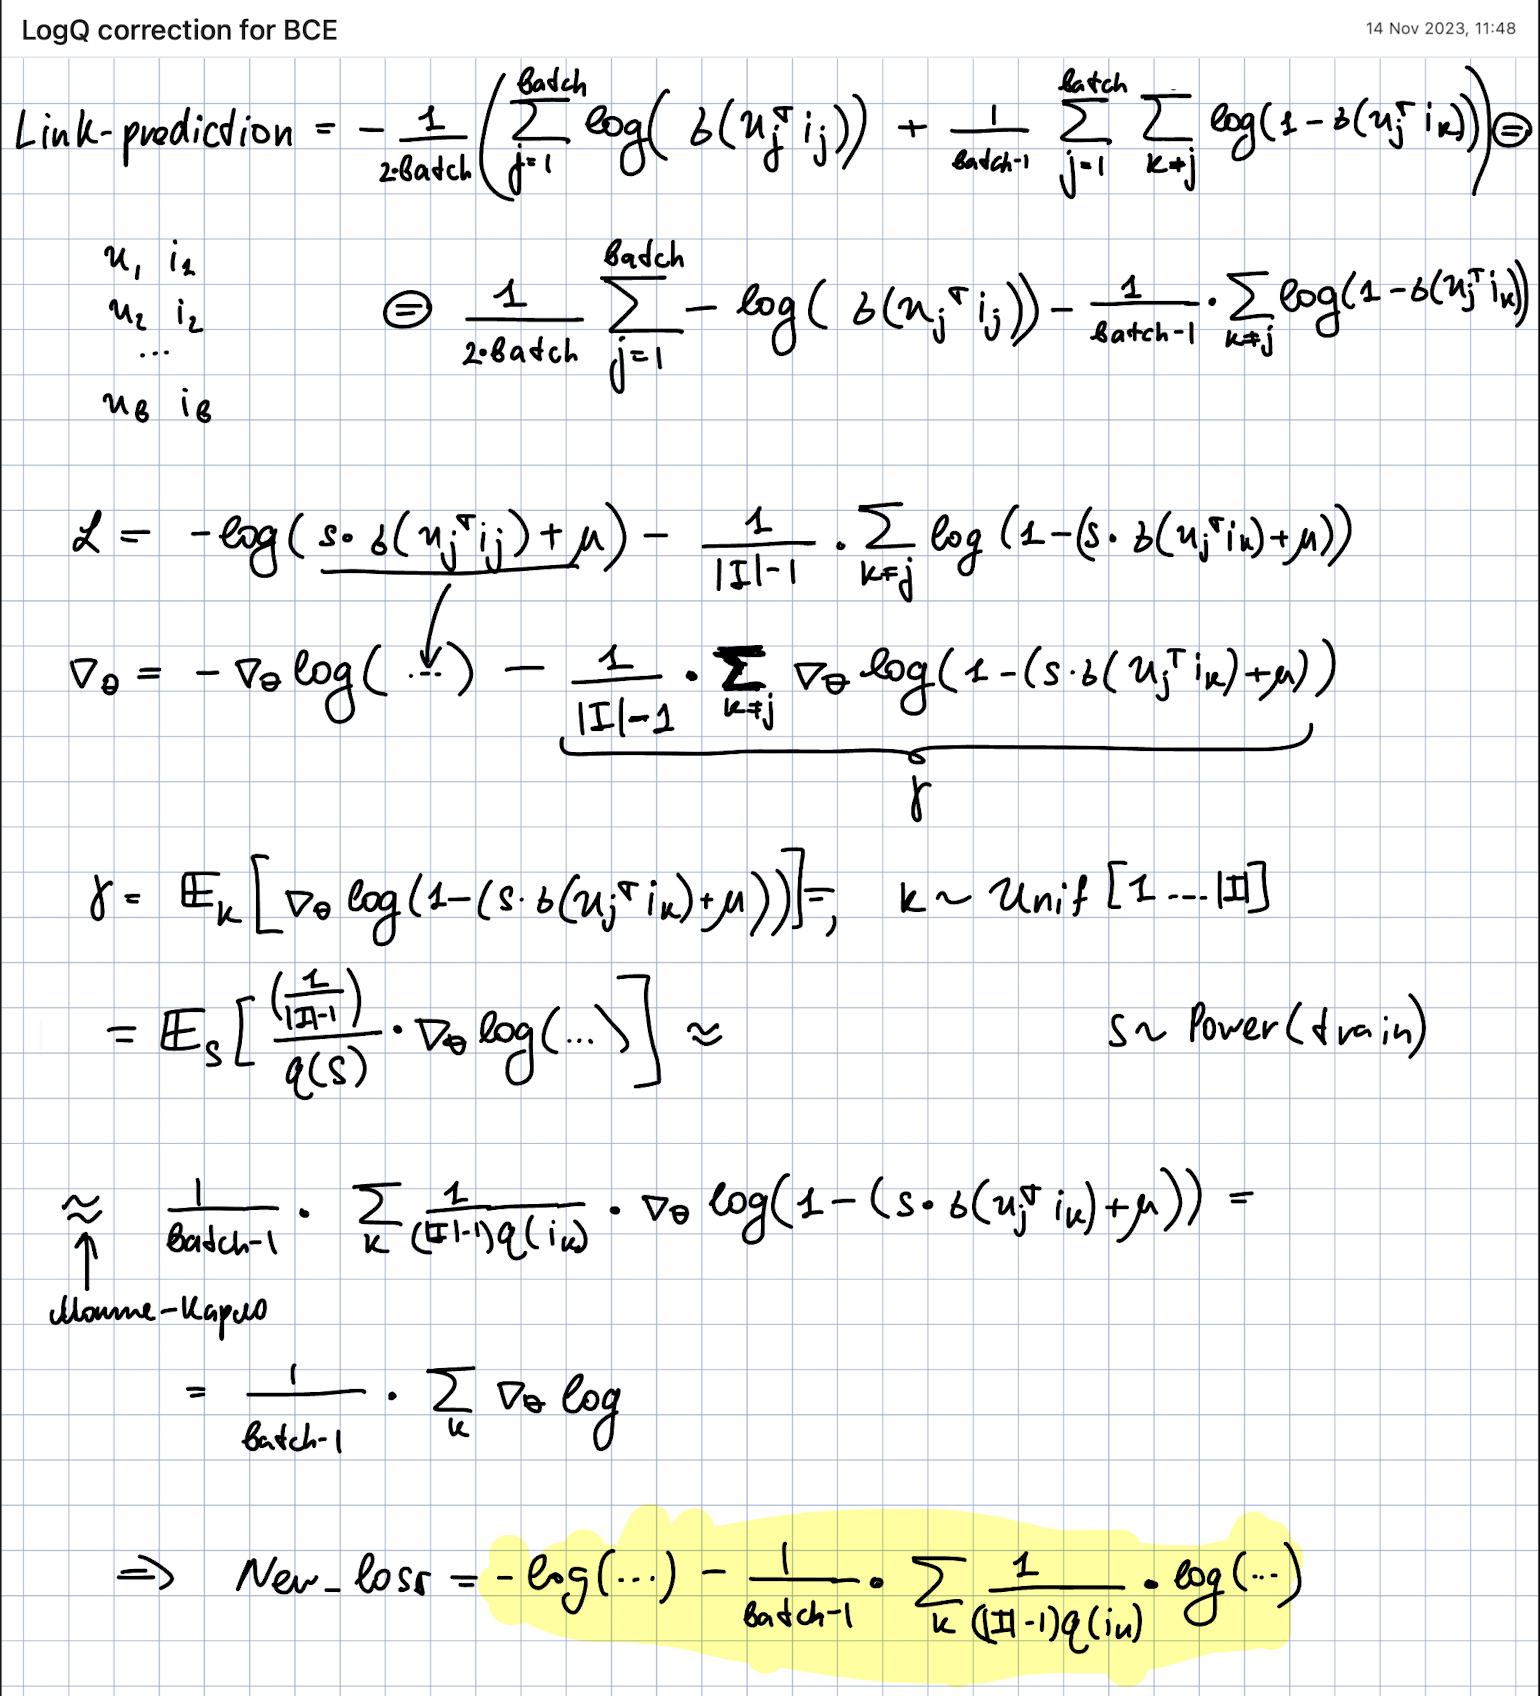
\includegraphics[width=130mm]{images/logQcorrection.png}
\end{figure}

\newpage
Получили первзвешивание по вероятностями.
\section{Эксперименты}

Эксперименты проводились на наборе данных MovieLense-1M. Статистики по набору данных представлены в 
таблице 1.

\begin{table}[h]
    \centering
    \rowcolors{2}{gray!10}{gray!40}
    \begin{tabular}{c|c|c|c}
        Dataset & Users & Items & Interactions\\
        \hline
        MovieLense-1M & 6,040 & 3,416 & 999,611 \\
    \end{tabular}
    \caption{Экспериментальные наборы данных.}
    \label{tab:my_label}
\end{table}

Для SASRec все параметры были взяти из оригинальной статьи \cite{sasrec}. Итоговые результаты представлены в таблице 2.

\begin{table}[h]
    \centering
    \rowcolors{2}{gray!10}{gray!40}
    \begin{tabular}{c|c|c|c}
        Model & Recall@1 & Recall@10 & NDCG@10 \\
        \hline
        SASRec & 0.043 & 0.232 & 0.135 \\
		GraphSASRec & 0.079 & 0.292 & 0.165 \\
    \end{tabular}
    \caption{Результаты.}
    \label{tab:my_label}
\end{table}

\section{Заключение}

Предложенный подход показал улучшение с точки зрения метрик ранжирования. NDCG@10 было увеличиено на 22 процента для задачи предсказания следуюещго взаимодействия пользователя.
Дальнейшие улучшения могли бы заключаться в рассмотрении сильно гетерогенных графов и более сложных архитектур графовых нейронных сетей.

\bibliographystyle{abbrv}
\bibliography{references} 

\end{document}